\chapter{Clinical Background}
\label{ch:clinical}

\section{Congenital Heart Defects}

Congenital heart defects and congenital heart disease (CHD) both refer to defects in the heart or the vessels around the heart which formed during  fetal development. Heart defects affect how blood moves into, through, and away from the heart. 
CHD can affect any combination of heart chambers and blood vessels with varying degrees of severity. The lesions prevent the cardiopulmonary system as a whole from functioning correctly, but pinpointing and treating the defects effectively can be a complex process.
 
% Causes of CHD: genetic syndromes, single gene mutations, environmental exposure, and unknown
There are a number of genetic and environmental factors associated with different presentations of CHD \cite{Mozaffarian2016}. Genetic conditions such as Down syndrome, Turner syndrome, 22q11 deletion syndrome, Williams syndrome, and Noonan syndrome are associated with different CHD presentations. Maternal behaviors such as smoking and binge drinking are known to cause heart problems in the fetus. Other maternal risk factors are obesity, folate deficiency, and living at a high altitude. Paternal exposure to phthalates, anesthesia, sympathomimetic medications, pesticides, and solvents may increase the risk of the fetus for developing CHD. While there are quite a few factors in this list, there are many CHD cases whose causes are unknown.

\begin{figure}
\centering
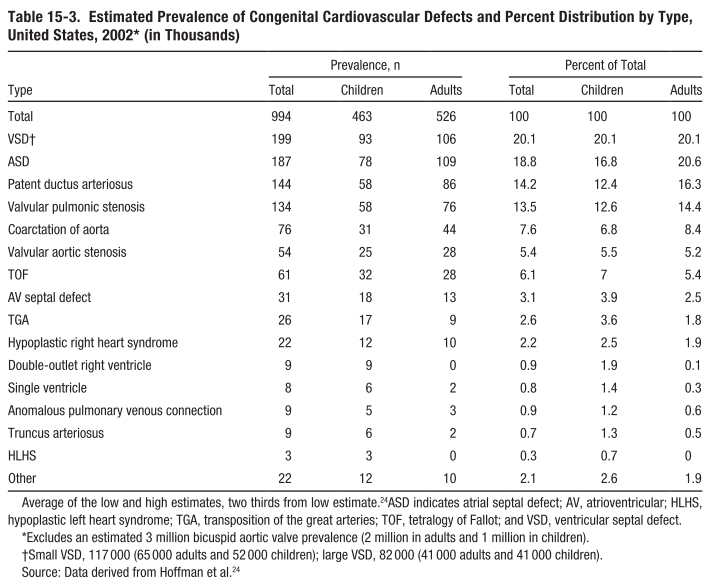
\includegraphics[width=0.6\textwidth]{3/chd-defects-usa.png}
\caption{Table of prevalences of congenital heart defects borrowed temporarily from \cite{Mozaffarian2016}.}
\label{ch2:fig:usa-defects-prev}
\end{figure}

% Diagnosis
The process of diagnosing CHD can begin before birth. A specialized ultrasound test called fetal echocardiography can detect heart abnormalities as early as the second trimester of the pregnancy. Additional tests, such as amniocentesis and follow-up ultrasounds may be used to determine treatment options before the patient is born. Generally, severe CHD cases present and are detected at earlier stages, but minor defects may not become apparent until the patient is older. Tests used to diagnose CHD in postnatal patients include electro- and echo-cardiograms, chest x-rays, pulse oximetry, exercise stress tests, computed tomography or MRI scans, and cardiac catheterization. Treatment of different defects varies from monitoring and medication to surgery and cardiac implants.

The incidence of CHD in live births vary across countries and continents. The United States reports approximately 4-10 CHD case per 1000 live births. Europe and Asia see about 6.9 and 9.3 CHD cases per 1000 live births \cite{Mozaffarian2016}. 
In China, the incidence of CHD ranges from 8.98 to 11.1 per 1000 live births \cite{Zhao2019} \cite{Qu2016}. 
A pair of studies from Iran report incidences of 8.6 and 12.3 per 1000 live births, though the studies note that they were performed in different geographical locations with different populations within the country \cite{Nikyar2011} \cite{Rahim2008}.
One report from Dharan reports an incidence of 5.8 per 1000 patients admitted to a tertiary care hospital over a 12 month period \cite{Shah2008}. A study of newborns at one hospital in New Delhi, India claims an incidence of 3.9 per 1000 live births, though this rate may be a poor estimate as there is a significant delay between patient birth and referral to a cardiac center in India \cite{Khalil1994} \cite{Saxena2005}.

These incidence rates should be analyzed with some caution. In many cases, the reported rates were based on medical records. Medical records are not always correct. Additionally, the only way for a person to have a medical record is for him to go to a medical center. Not everyone who has CHD is able to seek medical help, often because of their geographical locations or their income. Even if a patient is able to seek medical help, the availability of proper cardiac care varies between and within countries. 

As screening tools become more effective and more widespread, it is expected that incidence rates will increase as defects are detected earlier. Generally, the earlier a defect is detected, the earlier it can be treated. Early detection and treatment means more CHD patients will live to adulthood. Currently, Webb et al. estimate that at least 12 to 34 million adults have CHD, and this number is expected to increase \cite{Webb2015}.

It is important to note that each defect type has a different prevalence, a different treatment plan, and different expected outcomes. A breakdown of prevalence rates of some of the most common lesion types can be seen in Figure \ref{ch2:fig:usa-defects-prev}. % See (16)
Once a patient is diagnosed with one of these defects, the specific nature of his case must be clearly documented. The documentation of CHD using the International Classification of Diseases, Ninth Revision, Clinical Modification (ICD-9-CM) has 25 high level codes representing various presentations of CHD, but these codes used alone are often not sufficient for describing a patient's true condition \cite{Mozaffarian2016}. Additional ICD-9-CM codes should be used to communicate the finer details of a patient's condition. 

\begin{figure}
\centering
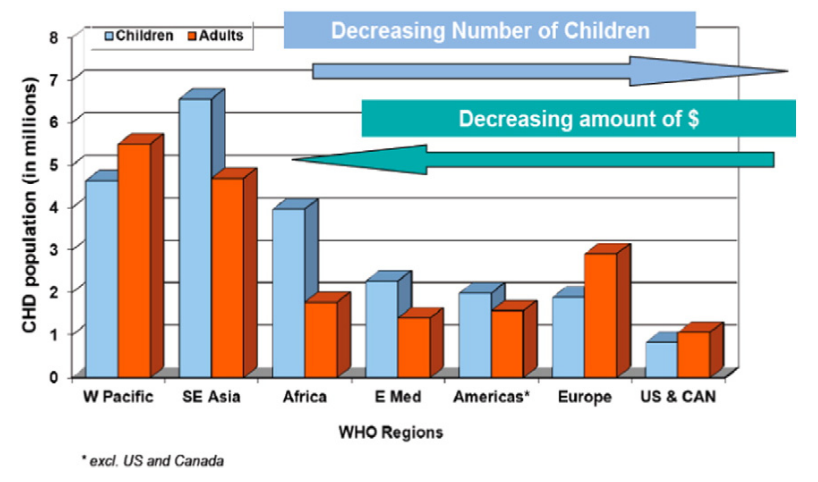
\includegraphics[width=0.7\textwidth]{3/CHD-burden-webb.png}
\caption{Estimated CHD burden in World Health Organization (WHO) regions using incidence rates of approximately 12/1000 and 4/1000 in children and adults, respectively \cite{Webb2015}.}
\label{ch2:fig:CHD-burden}

\end{figure}

%Depending on the cause of the 
The financial burden of CHD varies depending on the defect. Certain defects require complex, expensive surgical repairs while others can be treated with less expensive approaches \cite{Mozaffarian2016}. The burden of CHD across the globe was outlined by Webb et al. Their figure illustrating the prevalence of CHD and the availability of funds with which to treat it can be see in Figure \ref{ch2:fig:CHD-burden}. As the overall mortality of CHD declines, the burden of CHD is expected to increase \cite{Mozaffarian2016}.

% Complications and risks
Unfortunately, the cost of treating CHD alone is not the only burden a patient must undergo. Patients with CHD are also at increased risk for heart failure and infections \cite{Mozaffarian2016}. Children with CHD are at 19-fold risk for stroke compared to their healthy counterparts \cite{Fox2015}. In a study of Swedish citizens born between 1970 and 1993, Giang et al performed a study compared the prevalence of cardiac conditions in patients with and without CHD \cite{Giang2018}. They found that patients who had a CHD diagnosis were at about eight times higher risk for intracerebral hemorrhage and subarachnoid hemorrhage than their non-CHD counterparts. The CHD patients were also more likely to suffer from arrhythmia and heart failure.

% When are patients diagnosed?
% Expected lifespan
% Treatment plan
% Financial burden

\section{CHD and Neurocognitive Disorders}

Cardiac conditions are not the only complications CHD must deal with. In recent years, researchers have found that there is a relationship between CHD and neurocognitive disorders. 

\subsection{Causes}

Early research in this area focuses on the neurodevelopmental status of neonatal patients pre- and post-surgical intervention. One theory was that some factor or factors in the surgical intervention caused brain injuries in the patients. This idea proved to be inaccurate when researchers began detecting neurological malformations \textit{in utero}.

In a systematic review of available literature regarding prenatal and postnatal presurgical CHD cases and neurodevelopmental outcomes, Mebius et al. identify two theories about the causality of  neurodevelopmental delays and CHD \cite{Mebius2017}. The first theory is that abnormalities in the cardiac system prevent the developing brain from receiving enough oxygen and nutrients, which disrupts prenatal brain development. The second theory is that faulty genetic pathways used during both cardiac and brain development cause both conditions to co-occur. However, 11 articles Mebius et al. found during their review that are related to bloodflow through the umbilical artery suggest a third theory. During the prenatal period, a fetus receives oxygen from the mother via the placenta. If the placenta was not functioning correctly, it could lead to the fetus receiving not enough oxygen. Lower quantities of oxygen throughout prenatal development could potentially cause problems both in brain and cardiac growth. The 11 articles have contradictory results, but some researchers are currently investigating the role of the placenta in CHD and prenatal brain development.

%\subsection{Common Disorder Combinations}

\subsection{Aging}

Survival of CHD patients to adulthood has increased from 10\% to 90\% over the last several decades. The impact of the combination of CHD and neurological conditions throughout a patient's lifetime is starting to be explored. The aging of the CHD population has also sparked interest in the relationships between CHD and adult-stage neurological disorders such as dementia and Alzheimer's. 

%To address:
%\begin{itemize}
%\item Common combinations
%\item Joint treatment?
%\item Additional risks?
%\item Joint financial and emotional burden on caretakers? 
%\item CHD, neuro, and aging? Dementia/Alzheimer's? Recent data ... MIND neuroimaging ancillary r01 dec 17
%\end{itemize}

\section{Identifying Neurocognitive Disorders}

\subsection{Patient Surveys}

Surveys known to be used for studying the relationship between CHD and neurodevelopment are

\begin{itemize}
\item National Institute of Health Toolbox (3 - 85 years): ``Performance tests of cognitive, motor, and sensory function and self-reported measures of emotional function for adults and children in the general population and those living with a chronic condition''.

\item Sue Beers (4 - 18 years [not inclusive of 18 years]): WASI-II, NEPSY-2, WRAML-2, D-KEFS, WISC-IV, Grooved Pegboard, BRIEF, Beery-Buktenica VMI, ASRS, Conners-3, BASC-II, ABAS-II, PedsQL General, PedsQL Cardiac, Pictoral Scale Self Perception Profile.

\item SVR-III NDT (9 - 13 years [not inclusive of 13 years]): WIAT, NEPSY, WRAML, D-KEFS, WISC-V, Grooved Pegboard, BRIEF, Beery-Buktenica VMI, ASRS, Conners ADHD Index, BASC-II, ABAS-3, PedsQL General, PedsQL Cardiac

\item Bayley Scales of Infant and Toddler Development -III (1 - 24 months): Subtests include cognitive, language, social-emotional, motor, and adaptive behavior tests \cite{Mebius2017}.

\item Battelle Developmental Inventory (Birth - 8 years [not inclusive of 8 years]): Subsets include cognition, communication, social-emotional development, physical development, and adaptive behavior.

\item Developmental Assessment of Young Children (Birth - 6 years [not inclusive of 6 years]): Subtests include cognition, communication, social-emotional development, physical development, and adaptive behavior.

\item Preschool Language Scale + Receptive-Expressive Emergent Language (Birth - 3 years): Total language, auditory comprehension, expressive communication, articulation, receptive language, expressive language, and inventory of vocabulary words.

\item Peabody Developmental Motor Scales (Birth - 5 years): Subtests include reflexes, stationary, locomotion, object manipulation, grasping, visual-motor integration
\end{itemize}

The goal of these surveys is to compare the patient's cognitive function and neurological functions to expected milestones. Certain deviations from certain milestones are indicative of different disorders.

\subsection{Neurological Images}

When an area of the brain is active, it uses more oxygen than the surrounding regions. Functional MRIs (fMRI) are sensitive to signals emitted by deoxygenated hemoglobin. The blood oxygen level dependent (BOLD) signal recorded by the fMRI reveal regions of the brain which are active at the same time. These combinations of regions are called neuronal networks. 

Many neuronal networks exist, but most of them are considered to be task related. In 2001, Raichle et al. suggested the existence of a neuronal network which operated when a person is at rest \cite{Raichle2001}. Their theory was confirmed by Greicius et al. in 2003 \cite{Greicius2003}. Because the patient is not performing a specific task when they are in a resting state, the resting-state networks have the potential to reveal valuable information about a patient's neurodevelopmental status.

A fMRI taken of a patient in a resting, task-free state, is called a resting-state fMRI (rs-fMRI). rs-fMRIs are sequences of image volumes acquired over a period of a few minutes. The image volumes themselves have relatively low spatial resolution when compared to structural MRIs, but their temporal resolution is significantly higher as a new volume is acquired every two to three seconds. 

The BOLD signals in rs-fMRI image sequences are analyzed using a process called functional connectivity analysis. Functional connectivity analysis identifies patterns and networks of brain activity. Some functional connectivity analysis studies have lead to the discoveries of links between specific disruptions in these naturally occurring networks and neurodevelopmental diseases such as autism and attention deficit hyperactivity disorder \cite{Assaf2010} \cite{Zang2007}. With further refinements of both acquisition techniques and characterization of these functional networks, clinicians may be able to use rs-fMRI to evaluate the neurodevelopmental status of CHD patients and to identify patients who may benefit from certain therapies or neuroprotective interventions.

\section{Summary}

CHD consists of a variety of defects affect the vessels and chambers of the heart. It has a worldwide prevalence of about 8 per 1000 live births, meaning about 1.35 million children are born with CHD every year. Since the survivability of CHD has increased from 10\% to 90\%, the medical community is faced with a growing, aging population of CHD patients. Many of these patients also suffer from neurocognitive disorders that co-occur with CHD. The neurocognitive disorders are usually diagnosed using at least one of many psychological survey-based evaluations, but these methods are subjective. rs-fMRIs could be used to identify patients who have functional connectivity patterns associated with different neurocognitive disorders, and eventually may be used to identify patients who are at risk for developing these disorders.
%The next chapter will address the challenges of using rs-fMRIs as a tool for diagnosing CHD.
